\leadchapter{
The main part of this appendix chapter focuses on paper \autocite{desvaux_etal21}, in which we developed a new industrial, computational repurposing approach named \emph{Patrimony} and applied it to identify candidate therapeutic drugs that could help control the progression of severe inflammation during COVID-19. I summarised the key concepts related in the following graphical infographic, in \Cref{fig:infographic-patrimony}. 


\begin{figure}
     \centering
     \begin{subfigure}[p]{0.95\textwidth}
         \centering
         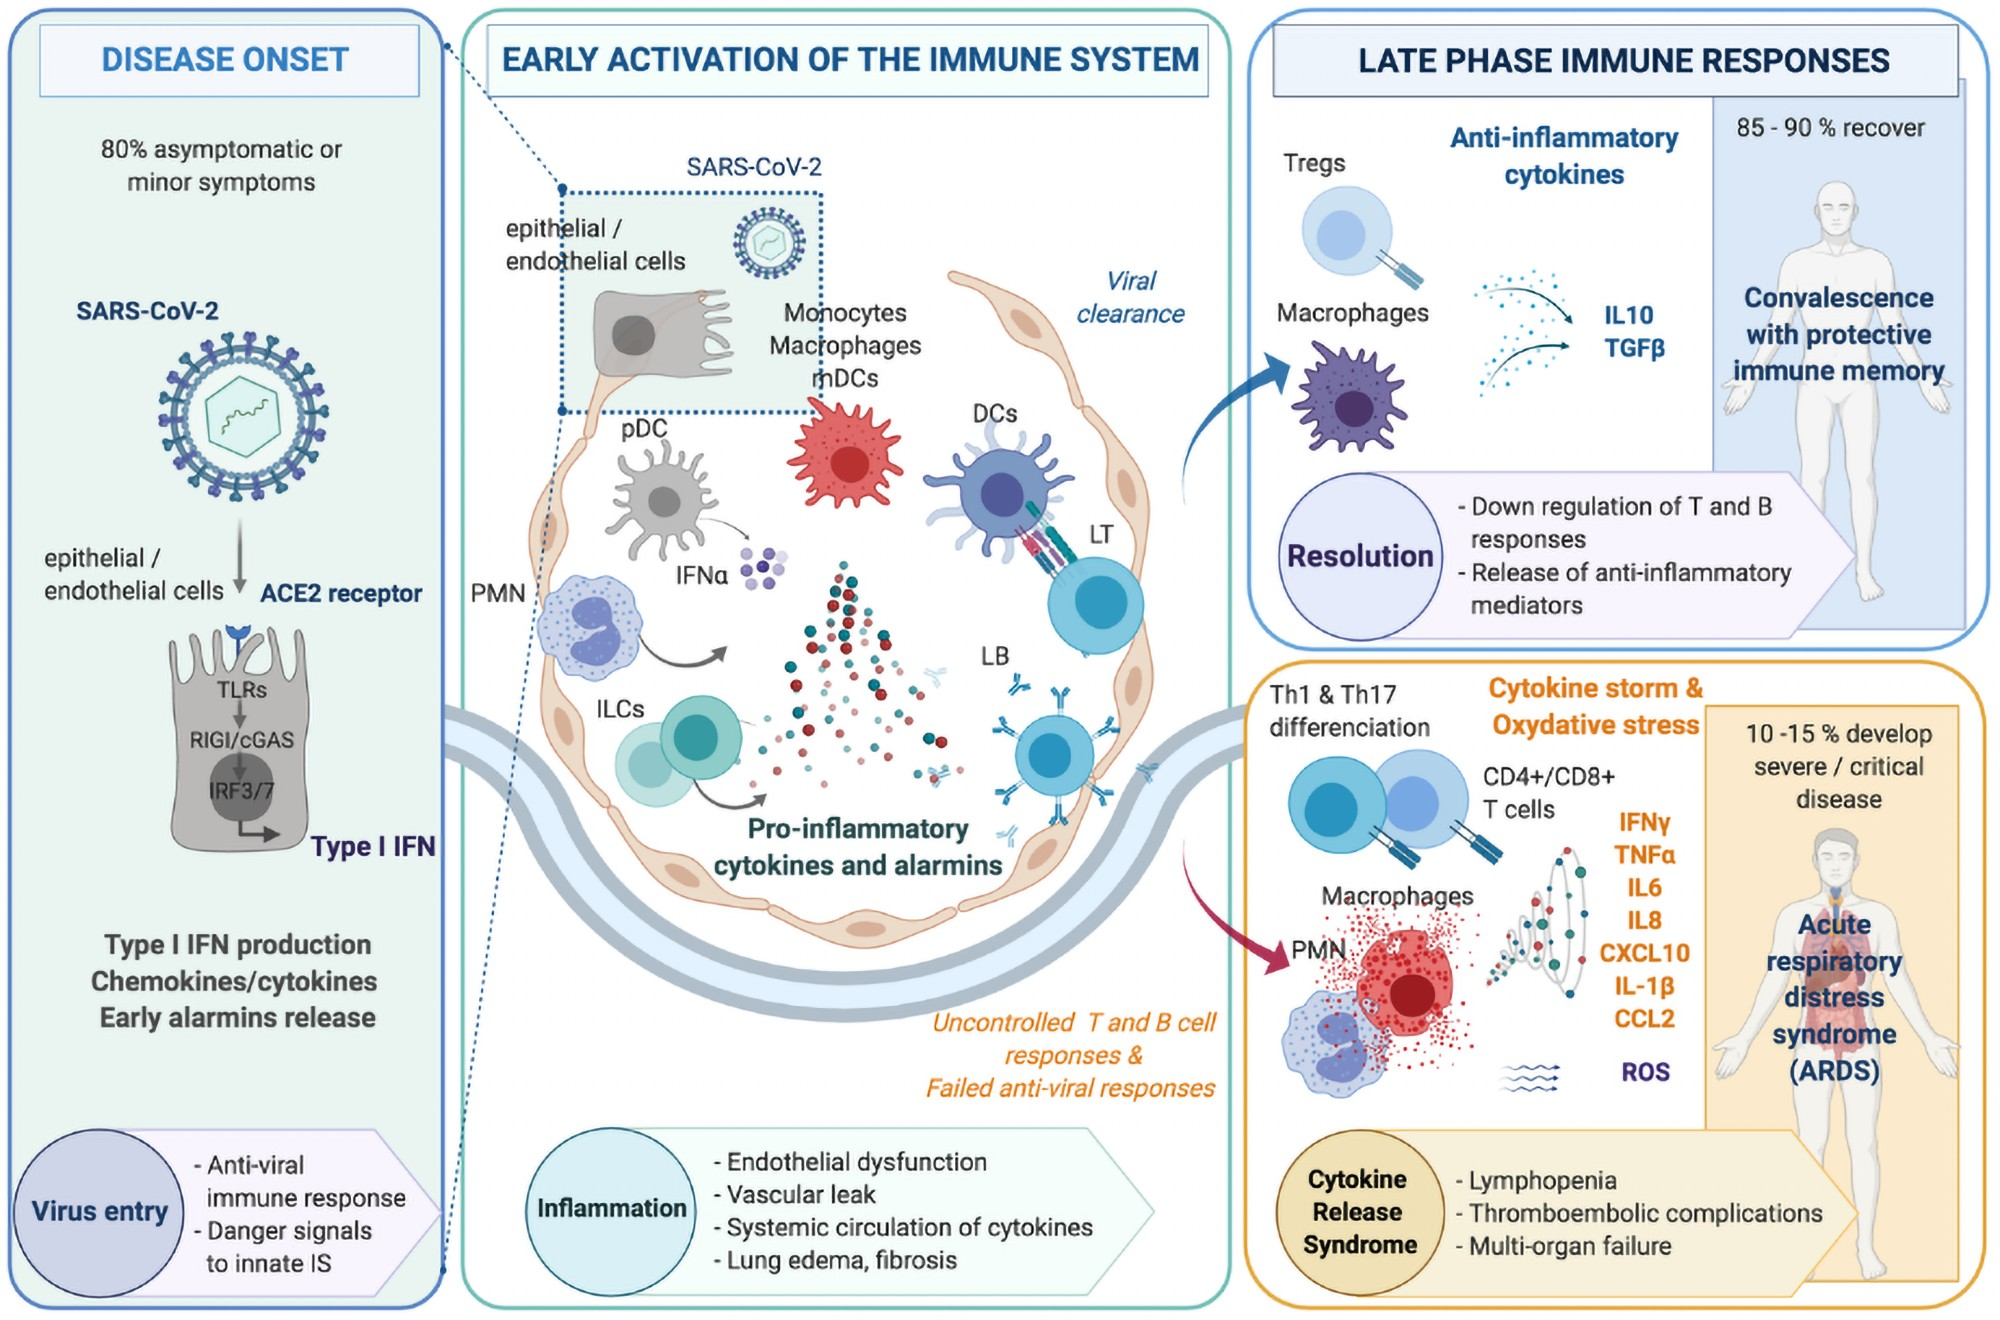
\includegraphics[width=\textwidth]{figures/repurposing/desvaux_2021_covid19_pathways.jpg}
         \caption[\textbf{The tree step progression describing the pathophysiology of COVID-19 in the airways.}]{See also \autocite[Fig. 1]{sumon_etal21} for a comprehensive list of possible drug targets to stop or decrease viral replication in infected cells.}
         \label{subfig:covid19-pathophysiology}
     \end{subfigure}
     \vfill
     \begin{subfigure}[p]{0.95\textwidth}
         \centering
         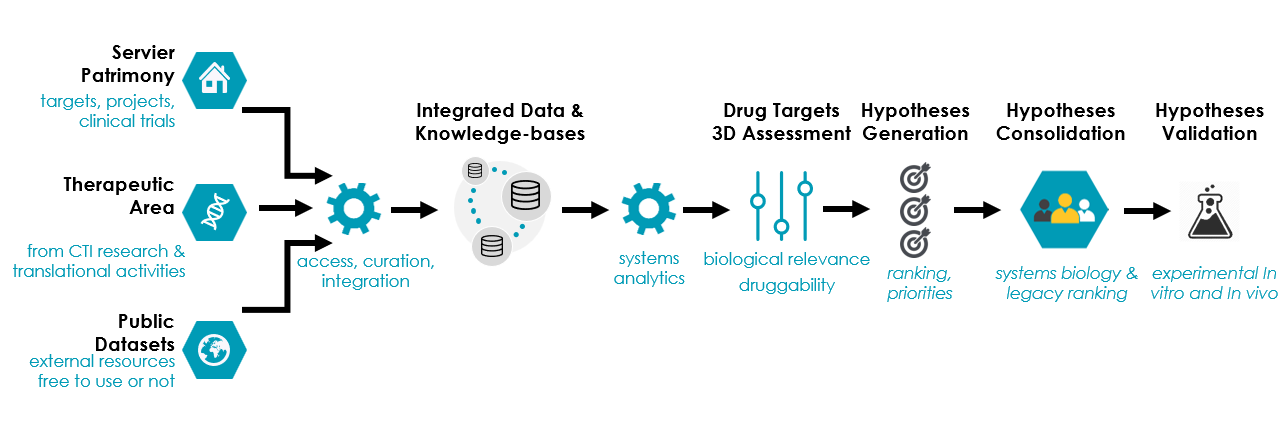
\includegraphics[width=\textwidth]{figures/repurposing/patrimony_industrialisation.png}
         \caption[\textbf{Patrimony general framework}]{Data sources are curated and integrated into a knowledge graph, refined with additional omics sources for each disease. Finally, several mining algorithms are used to evaluate the biological relevance and druggability of putative targets (infographic mostly inspired from \autocite[Fig.1]{guedj_etal22}.}
         \label{subfig:patrimony-industrialisation}
     \end{subfigure}
     \begin{subfigure}[p]{0.95\textwidth}
         \centering
         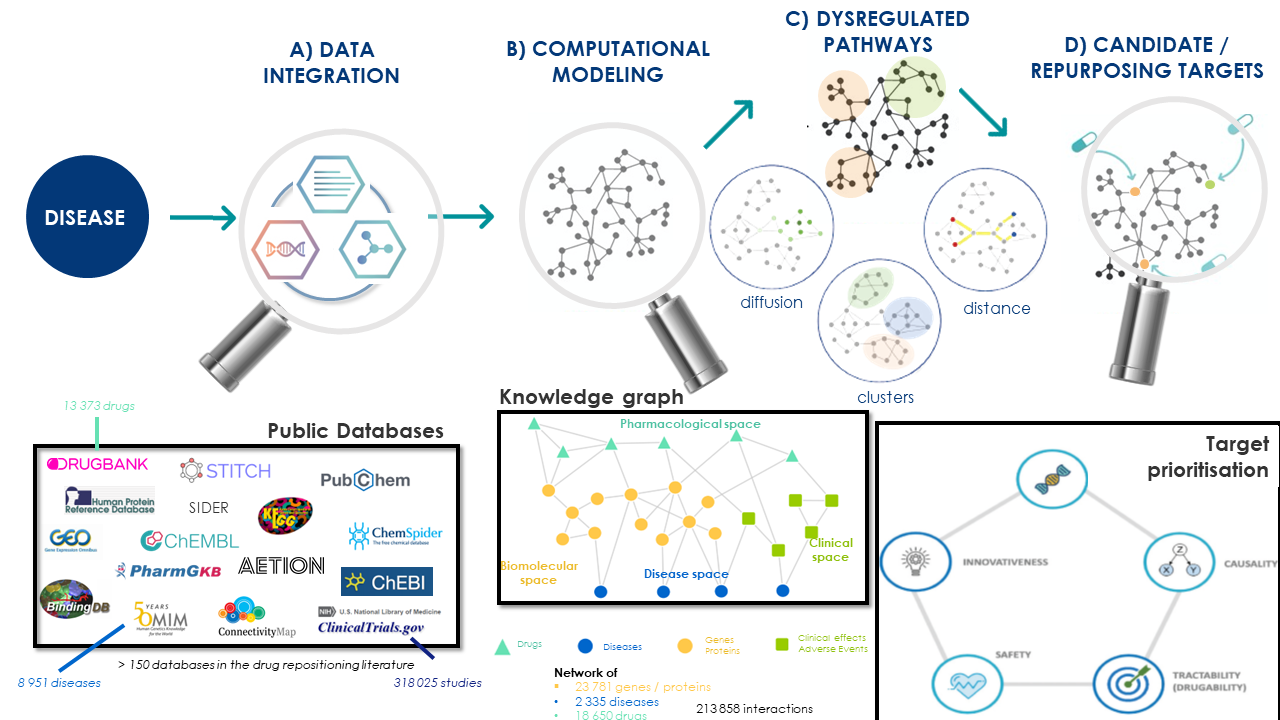
\includegraphics[width=\textwidth]{figures/repurposing/patrimony_repositioning_platform.png}
         \caption[\textbf{Main steps of computational medicine, up to drug repurposing, integrated within the Patrimony platform}]{Once data sources are curated and properly annotated, they are fused together through a relational diagram to build the Patrimony \enquote{knowledge graph}, encompassing biomolecular, pharmacological, disease, and clinical datasets. Subsequently, different approaches are used to mine the knowledge graph, for instance, to identify key driver genes or clusters of highly-interconnected entities. Ultimately, targets related to dysregulated phenotypes are ranked and prioritised through a global score aggregating five distinct dimensions, and the selected targets are returned with graphical ID cards to be easily read by end users, in particular biologists (infographic mostly inspired from \autocite[Fig.2 and Fig.3]{guedj_etal22}).}
         \label{subfig:repositioning-platform}
     \end{subfigure}  
    \caption{Infographic of Appendix C, about a proof-of-concept of our internal computational platform \enquote{Patrimony}.}
    \label{fig:infographic-patrimony}
\end{figure}


Indeed, the COVID-19 pandemic, caused by SARS-CoV-2 strain virus, leads to millions of hospitalization in intensive care, with an estimated requirement of ICU transfer ranging from $5\%$ to $32\%$ with respect to the country, \num{768560000} confirmed cases worldwide and \num{6951000} deaths, according to the most updated statistics provided by the world health organisation by July 2023 \autocite{abate_etal20}. And at the time we published the paper, no current approved FDA medication nor vaccine were widely available, while there were strong concerns about the effectiveness of vaccines against emerging new variants of the virus.


Practically, we focused on repurposing therapeutic drugs addressing severe lung inflammation caused by COVID-19, since most patients with Covid19 die from \acrfull{ards}. But first, let's introduce briefly the general pathophysiology of COVID-19 in the airways, as displayed in \Cref{subfig:covid19-pathophysiology}. Disease evolves in three steps: first, viral infection of cells presenting the ACE2 receptor triggers the production of IFN$\alpha$ by plasmacytoid dendritic cells (pDC) (left panel in \Cref{subfig:covid19-pathophysiology}, see also \Cref{subsec:collab-innate-adaptive} for detailed explanation about the cooperation between the innate and adaptive immune system). Second, the release of interferon molecules activates an inflammatory stage, where infected cells interact with immune cells (macrophages and innate lymphoid cells), leading to the release of pro-inflammatory molecules (center panel in \Cref{subfig:covid19-pathophysiology}), which in turn triggers the adaptive immunity, involving the recruitment of CD4+ T cells and CD8+ T cells that target infected cells, and on the other hand the release of antibodies neutralising viral antigens. The last stage, named \enquote{late inflammatory phase} comes along with two possible outcomes: in $85-90\%$ of the patients, inflammation is modulated by down-regulating effector T and B cell through the release of anti-inflammatory mediators (right upper panel, in \Cref{subfig:covid19-pathophysiology}), while in $10-15\%$ of patients the inflammatory response does not relapse (persistent T cell activation and myeloid cell activation, cytokine storm, oxidative stress, \ldots), leading ultimately to extensive tissue damage and \acrshort{ards} (right lower panel in \Cref{subfig:covid19-pathophysiology}).



To identify driver proteins and transcriptomic pathways involved in the severe cases of Covid19,  we have collected in a first time various public gene expression data from both SARS-CoV-2 infected and control pulmonary cells \footnote{We leveraged two distinct cell lines: bronchial epithelial (NHBE, \autocite{blanco-melo_etal20}) and human lung epithelial cancer (Calu-3, \autocite{ackermann_etal20}) cells} and then identified proteins significantly related with early lung inflammation and the severity of cytokine storm events \autocite{merad_martin20}. 
After a comprehensive pre-processing step, which included removing outliers and discarding genes with low expression, we ran standard \acrfull{dgea}, comparing the COVID-19 batches with the mock batches. The inferred list of differentially expressed genes was then provided as input to the \acrfull{ipa} software \autocite{kramer_etal14}, which in turn returned molecular pathways deregulated by lung inflammation. Notably, we classified arbitrary these genes into two categories, related to their biological function: \enquote{Alarmins}, immunomodulatory proteins which recognise molecular damaged patterns from injured cells and display them to activate a bunch of innate immune cells (see \Cref{subsec:innate-system}) and \enquote{Cytokine storm}, gathering mostly cytokines promoting the severe inflammatory response observed in many COVID-19 patients. 

The identification of new drug targets itself was performed through two complementary drug repurposing strategies:

\begin{itemize}
\item In the network-based approach to drug repurposing, we capitalise on the existing integrated network of \acrshort{ppi} of \autocite{cheng_etal19}, compiling \num{15894} distinct proteins with up to \num{213861} significant pairwise interactions, all derived from a compendium of 15 distinct protein databases. We then fused this integrated network with two drug target databases:  the Therapeutic Target Database (TTD, \autocite{chen_etal02}) and Drugbank \autocite {wishart_etal08}, gathering \num{3092} drugs. The \emph{network proximity} between disease-related proteins and drug targets within the PPI network was used as proxy of the relevance of drugs to the disease. Measure similarity was estimated through two complementary metrics: a \emph{topological distance} and a \emph{diffusion-based} distance, the first one returning the averaged shortest path length between the disease-related proteins and the drug targets and the second quantifying the similarity of the perturbations induced on disease-related proteins by biological mechanisms dysregulated by the Covid-19 on one side and drug targets on the other. The second metric is largely inspired from the Diffusion State Distance (DSD, \autocite{cao_etal13}), a proven \emph{metric} \autocite[Lemma 1]{cao_etal13} that leverages asymptotic random walk transition probabilities to estimate the distance between two nodes \footnote{This metric has some interesting asymptotic properties, notably proof of asymptotic convergence \autocite[Lemma 2]{cao_etal13} and even derived explicit form in the limit \autocite[Claims 2 and 3]{cao_etal13}.}. Then, for each metric used, bootstrap distributions for nodes having the same degree in the graph were computed to derive $p$-values, then combined using the Fisher's probability test and finally the drugs were ranked by decreasing order of aggregated $p$-value.

\item To strengthen the connectivity findings, we then take profit of the Connectivity Map (Cmap, \autocite{lamb_etal06}), perturbagen database, which aggregates more than \num{3000} compounds known as distributing the transcriptomic expression. We then compute Cmap scores (compiling different comparison methods, we determine that Pearson correlation was the most robust and reproducible one for our experiment) reflecting the potential therapeutic effect of each of the listed perturbagen. Indeed, the core idea underlying the use of connectivity maps is to extract a set of perturbagens displaying a reversed gene expression profile, a negative correlation metric being an indicator of a reversed profile and accordingly a suggested therapeutic indication of the perturbagen.
\end{itemize} 
}

\chapter{Network-based repurposing applied to Covid 19}
\label{chap:covid19}

\section{Drug repurposing: a brief historical overview}
\label{sec:drug-repurposing}

\paragraph{Overview: Drug Development Process}
\label{para:drug-development}

Drug development is an essential process for the discovery and availability of life-saving and life-improving medications. However, from the identification of potential biological markers to post-marketing surveillance, it is also a complex and challenging journey with numerous obstacles and failures. Throughout this process, pharmaceutical companies face various setback, with many drug candidates failing at different stages due to issues with efficacy, safety, or lack of sufficient clinical evidence. In addition, the experimental, human and computational burden deter numerous small companies into developing their own molecules, instead relying on the resiliency of bigger pharmaceutical groups. 


While the ancestry of each successfully developed drug is quite unique, most of them follow generally the following storyline development (\Cref{subfig:drug-pipeline}):

\begin{enumerate}

\item The first phase is \emph{Discovery and Target Identification}, where researchers identify potential drug targets (e.g., proteins, enzymes, receptors) that are involved in a disease process, leveraging high-throughput screening, omics combined with prior knowledge or literature review  techniques to identify ligands interacting with these targets. The next stage consists of selecting the most promising drug candidates, termed \enquote{lead compounds} that interact with the target, displaying both strong molecular activity and specificity towards the target. Numerous steps make up the \emph{early drug discovery}, that for obvious reasons of brevity, we can not detail in this section. We hence recommend the interest reader the reading of \autocite{hughes_etal11}, which encompasses the description of the key preclinical stages, ranging from initial target identification and validation, through assay development, high throughput screening, hit identification, lead optimization up to the final selection of a reduced subset of candidate molecule for clinical development.

\item Before testing on humans, the selected lead compounds undergo extensive \emph{preclinical testing}, which involves in-vivo testing on animals, in-vitro testing on cell lines and recently in-silico simulations, with the development of \enquote{twin models} expected to reproduce the complexity of the highly connected biological mechanisms, with extensive safety assessments to evaluate the drug's efficacy, toxicity, and pharmacokinetics.

\item Following the Investigational New Drug Application to the regulatory authorities (e.g., FDA in the US), ascertaining the validity of the preclinical testing and outlining the human clinical trials, there is the most critical phase of drug development, since it involves human patients and enables the final commercialisation of the drug. This step generally decomposes in three stages:

\begin{itemize}
\item  Phase 1: Small-scale trials on healthy volunteers to assess safety, dosage, and side effects.
\item Phase 2: Trials on a larger group of patients with the target disease to evaluate efficacy and safety further, in some cases further splinted into a step a) to evaluate the pharmacokinetics and a phase b) to evaluate the pharmacodynamics. 
\item Phase 3: Large-scale trials involve a much bigger human cohort, to confirm efficacy and safety and monitor on the other hand any rare side effects.
\end{itemize}

\item If the results from Phase 3 trials are favourable, a New Drug Application is submitted to the regulatory agency for approval to market the drug, which, after conclusively stating the drug's benefits outweigh the risks for its intended use, approve the drug for marketing and use by the public.

\item The process does not stop once the drug enters the market, indeed, its safety and efficacy are continuously monitored through post-marketing surveillance, notably to detect any adverse reactions or long-term effects. This phase has gained recently increasing interest, related to horrendous clinical scandals, as well as the enumeration of side effects may help towards the development of repositioned drugs, with new indications, or suggest more efficient combination of therapies as detailed in next \Cref{para:drug-repurposing-motivation}. The commercialisation, the study of the side effects and the potential additional therapeutic use cases describe the \emph{Life Cycle Management}.

\end{enumerate}

Even after successful completion of clinical trials and regulatory approval, drugs previously approved might be ultimately withdrawn from the market, resulting from post-marketing surveillance that detect unveiled drug's toxicity or introduction of a new compound with undeniable efficiency, one of the most controversial case hitting recently the headlines certainly being the Mediator health scandal \autocite{Mediator21}. However, even failures help researchers and industrials into refining their approaches, while potentially suggesting new  therapeutic uses, within a drug repurposing strategy (see \Cref{para:drug-repurposing-motivation}).

\paragraph{Motivation for drug repurposing}
\label{para:drug-repurposing-motivation}

The main purpose of drug repurposing is to identify existing drugs, generally clinically approved for a given medical use case, but displaying additional therapeutic value for other diseases or conditions. Determining new biological applications of existing drugs reveal paramount, since, despite increasing investments, the number of newly released molecules keep on decreasing.

Thereby, by determining new drug use case, repositioning is expected to speed up the drug development process, avoiding to reproduce the pharmacokinetics studies, and to reduce the sky-rocketing costs of drug development, compared to design molecules from scratch. Finally, and of utmost significance, the attrition rates are expected to significantly decrease, notably when anterior early-stage trials were conducted and positively evaluated the risk of safety failure. \autocite{nosengo16} has estimated that the average cost of introducing a repurposed drug to the market is approximately $300$ million dollars, against on average around $2-3$ billion dollars for a new molecule. In addition, the development process to release a new drug on the market has been estimated to 15 years while promising candidates undermined within the exploratory phase undergo a strikingly dropout rate of $90\%$ reaching Phase II clinical trials, mostly due to safety worries or inadequate effectiveness. This pattern of decreased \acrshort{RD} efficiency, gauged by the count of new drugs delivered to patients for each dollar expended and which decreased by half every 10 years since 1950, is commonly known as Eroom's Law, or the \enquote{valley of death}, illustrated by the attrition funnel diagram in \Cref{subfig:drug-pipeline}. This trend contrasts with the familiar Moore's Law that describes the exponential growth in computational power per unit of surface on a microchip over time.

Notably, such approaches are particularly relevant to provide novel treatment options for \emph{orphan diseases}, rare affections with still unmet medical needs, or in case of emergency, such as outbreaks like the COVID-19, for which the standard drug development process storyline is not adjusted \Cref{para:drug-development}.


Historically, many drug discoveries were accidental. For example, sildenafil citrate was originally developed as an antihypertensive drug, but then successfully repurposed to treat erectile dysfunction \autocite{ycharts}, an opportunistic process commonly known as \gls{serendipity}.
Yet, the recent fast accumulation of organised biomedical and omics datasets, coupled with innovative computational methods, have promoted the development of \enquote{data-driven} approaches. By analysing and integrating various types of data (e.g., chemical structure, omics, electronic health records, \ldots), such approaches have identified numerous candidate drugs and targets in an agnostic manner, uncovering unforeseen and unexpected connections between diseases and therapeutic compounds (see \autocite[Table 1 and Box 1]{pushpakom_etal19}, for a comprehensive review of repurposed drug success stories). 


\paragraph{Data-driven repurposing strategies}

Notably, data-driven approaches are classically separated between experimental and purely computational, data-driven strategies, the latter being subdivided into the following categories: 

\begin{itemize}
\item \emph{Signature matching} is the process of comparing the unique characteristics, such as transcriptomic, structural, or adverse effect profiles, all combined composing the so-called drug or disease \enquote{signature}, with those of another drug or disease phenotype. Transcriptomic signature can be used to unravel novel drug-disease and drug-drug associations, aiming to identify shared mechanisms of action between dissimilar drugs, alternative drug targets and/or potential off-target side effects. The underlying approach of this computational method relies on the \emph{signature reversion principle}, where it is assumed that a drug displaying a reverse transcriptomic profile can counterbalance the dysregulated expression patterns making up the hallmark for a given disease phenotype. In other terms, we hypothesise that an opposite drug signature should shift back the abnormal profile towards a healthy state (see \Cref{subfig:repositioning-strategies}, blue section). Chemical signature matching involves comparing the chemical composition of drugs with molecular patterns or sequences known for their biological activity. These approaches rely heavily on publicly accessible gene expression data, the largest and most famous one being certainly the Connectivity Map (cMap) project \autocite{lamb_etal06}, \autocite{lamb07}, and are largely inspired from previously developed \enquote{pathway
enrichment analysis} methods \autocite{zhao_rhee23} \autocite{subramanian_etal05} \autocite{lamb_etal03}. 

\item \emph{Biomolecular or pathway network-based approaches} involve studying the impact of drug or disease on omics networks, based on gene expression patterns, protein interactions or \acrfull{gwas}. The main purpose is to identify key gene drivers, through genetic variant information combined with tissue-specific interaction networks, that could either mitigate downstream the dysregulation pattern induced by disease-related mechanistic disorders, or used upstream as a biomarker indicator of the efficiency of a treatment. For instance, the perturbation analysis of gene expression data induced by respiratory viruses led in study \autocite{smith_etal12} to unravelling 67 common biological pathways associated with respiratory viral infections, which were ultimately checked against the DrugBank database to identify drugs targeting host-viral interactions (see details in \Cref{subfig:repositioning-strategies}, red section).

\item \emph{Clinical and side-effects databases}, either retrospective or undergoing, such as electronic health records (EHRs), post-marketing surveillance data and publicly available clinical trial data, has led to numerous drug repurposing successes, since the phenotypic effect observed is straightforward compared to the previously described methods. However, a systematic approach for analysing clinical data may provide additional drug repurposing opportunities, by not only considering explicit repurposing strategies, but also eliciting intricate similarity drug patterns by considering as well adverse effects \footnote{This principle of matching drugs based on indirectly shared side-effects, or diseases by similar drugs, is known as \enquote{guilt-by} association, see \autocite{paik_etal15} and \Cref{subfig:repositioning-strategies}, green section, for practical examples}. Among them, EHRs offer the most comprehensive source of information to identify drug-disease or drug-drug associations, however, leveraging these resources reveal a highly challenging task, including ethical and legal obstacles related to personal health records and painstaking extraction of highly unstructured information.
New natural language processing (NLP) combined with efficient computational power and alleviated open access from companies and governments to these health records could nonetheless keep pace of drug repurposing based on clinical trial and pharmacovigilance studies (\autocite{paik_etal15} and \Cref{subfig:repositioning-strategies}, green section).

\item \emph{Molecular docking} predicts binding compatibility between a ligand (e.g., a drug) and a target receptor (e.g., a protein, see \Cref{subsec:collab-innate-adaptive} for ligand and receptor definition). This technique can thus be used to identify potential drug-receptor interactions but further development of the tool is hindered by missing 3D structures for certain proteins \autocite{huang_etal18}, inconsistent target databases, and limited prediction ability, notably in detecting emergent \emph{entropic forces} occurring at the total molecular system \autocite{pagadala_etal17}.

\item The number of \emph{Genome-wide association studies} highly increased in the recent years, with a common goal of identifying genetic variants linked to specific disease traits. Interestingly, it turns out that the genes highlighted by GWAS studies, are more likely to code for \enquote{druggable} proteins, and thereby, supply potential targets for drug development. Furthermore, the continuous discovery of new gene variants and functions contributes to a enhanced and dynamic understanding of the biological mechanisms, concurring altogether to maintain the homoeostasis of the human genome \autocite{sanseau_etal12}.
However, setting apart gene variants that have a causal effect on disease phenotypes from spurious relations is a highly intractable task, especially in gene-rich loci displaying strong \gls{linkage-disequilibrium} \autocite{wang_zhang13}. 

\item Finally, large-scale in vitro drug screens paired with genomic data (\emph{pharmacogenomic interactions}), EHR-linked large biobanks and self-reported patient data, are promising avenues and databases sources for drug repurposing. For instance, human cancer cell lines (CCLs, \autocite{huang_vakoc16}) have been used to test the impact of hundreds of compounds on cell viability and thereby identify molecular characteristics of the cells related to drug response. Recent studies showed thus recently that CCL datasets were able to clinically replicate pharmacogenomic interactions of primary tumors, and among newly discovered interactions relating drugs to tumoral cell lines survival, many involved drugs already used against distinct types of cancer. Specifically, this higher resolution up to the genomic and cell type level can contribute to personalised cancer therapy, by targeting groups of patients displaying specifically identified genomic variants associated with stronger drug response \autocite{iorio_etal16}.
\end{itemize}

In addition to these data-driven approaches, machine learning methods promote the development of high-throughput experimental techniques, including \emph{phenotypic screening}, in which the idea is to rapidly test a vast amount of putative compounds and subset those with a specific phenotype \autocite{iljin_etal09}, and \emph{binding assays}, to identify novel target interactions from known drugs, using proteomic methods such as affinity chromatography or mass spectrometry \autocite{alshareef_etal16}. It is important to acknowledge that all these methods, compiled in \Cref{subfig:repositioning-strategies-general}, are now increasingly utilised in synergy as they are complementary.


However, a bunch of barriers related specifically with drug repurposing, including patent licenses, regulatory considerations and pharmaceutical organisational hurdles, hinder further development of computational or experimental repositioning. Legally approved drug patents are required to obtain the market exclusivity for drugs and thus ensure the economic sustainability of its commercialisation. However, repurposed drugs pose specific challenges: indeed, to register a new drug therapeutic indication (termed new method-of-use, MOU), you must enforce that the new repurposed use is innovative enough, leading thereby to early removal of promising candidates, since their extensive use was already described in the scientific literature.

Repurposed drugs with an orphan indication display a stronger potency of patent, since the EU approves 10 years of market exclusivity. However, in other disease cases, data exclusivity does not generally hold for other indications relying only on variations to existing marketing authorisations, while in the US, a new use of a previously marketed drug receives only 3 years of data exclusivity, a period usually not sufficient to recover the investment costs. Finally, off-label use of generic repurposed drugs does not always promote their commercial value, consider for instance a drug originally developed to cure for cancers, repurposed to cure common diseases \autocite{murteira_etal14}. 

The heterogeneity and the scattering of the available data across several companies and countries, on par with the requirement of innovative machine learning and network-based methods, promote stronger collaboration between small biotech firms, academic communities and big pharmaceutical companies. For instance, initiatives like the AstraZeneca Open Innovation Platform or the Pfizer's Centers for Therapeutic Innovation \autocite {ashburn_thor04} endorse external collaborations, yet, challenging data management arise when the repurposed indication falls outside the company's disease area, the development of the compound has been long stopped or no cured repository of the known side effects or parmacokinetics of a drug exist.

%\section{Enrichment analysis for the identification of pathways}
%
%\subsection{Fisher's exact test}
%\subsection{Gene set enrichment analyses (GSEA)}

\section{Introduction to the Patrimony initiative}
\label{sec:patrimony-overview}

To handle the ingestion of the ever-increasing data generated from genetics, multi-omics, molecular interactions or real-life evidence sources, pharmaceutical industries are increasingly developing dedicated computational environments, with the final purpose to identify both disease targets and promising drugs, in other words, to facilitate decision-making in drug development based on agnostic and data-driven approaches. Computing platform encompasses hardware, software and user interface components, while integrating diverse biomedical databases. 
While existing public or public-private initiatives, like Open Targets \autocite{koscielny_etal17} (reach an extensive description of consortium projects in \autocite[Supp. Table 2]{guedj_etal22}), were already implemented, and after an extensive benchmark on external solutions and examination of projects from numerous start-ups, my former manager decided to implement a corporate computational solution, offering reactivity, flexibility, better integration of internal data sources and relapsing legacy concerns. To that end, the Computational biology team, whom I am an active member, contributed to the implementation of the high-throughput computing platform \enquote{Patrimony}, so called since we capitalise on both proprietary and public data to foster innovation and decrease the strong attrition rates in drug development \footnote{Servier has not released any new drug on the market, nor receive additional NDA for 15 years, and its sale margins are comparable to those of generic drug company, which, by definition, only rely on existing drugs \autocite{guerre16}.}.


The development of this computational platform involves first identifying and curating relevant data sources, both in-house and public, to integrate them into an uniformised knowledge graph. Then, machine-learning algorithms combined with graph theory were developed to mine the network. Finally, we adjust the platform by supplementing it with application-specific add-ins, tailored to the disease of interest, including immuno-inflammatory, oncological or even neurological disorders. This whole process is summarised in \Cref{subfig:repositioning-platform}, ranging from data acquisition to experimental validation, through hypothesis generation and target prioritisation.

The proprietary knowledge graph  underlies the core of Patrimony, by displaying in a compact and interpretable structure a wide set of entities and their relationships. To explore the resulting complex network, we applied different techniques from the graph theory and statistical field, which enable to identify \emph{hubs} (key driver genes displaying a high degree) and \emph{clusters} (highly interconnected cliques of vertices) within the graph or measure using an integrative and connected approach the impact of a drug or a disease on the biological pathways, benefiting from various diffusion and propagation algorithms \footnote{One of the main challenge in developing a relevant similarity metric is underscored by the \emph{hub protein bias} \autocite{fiscon_etal21}, occurring when key driver proteins display a high degree = high level of pairwise connections in the network, while strong sparsity is generally required to generate discriminatory metrics. Contrary to common beliefs, it was discovered that the distribution of the degree of vertices, i.e., the number of connections per gene or protein, did not follow a \emph{scale-free} hypothesis, in other words, that the number of highly-connected genes was not significantly smaller than the number of weakly-connected regions of the graph \autocite{broido_clauset19}.}. Furthermore, a distance value alone is not meaningful, as highly dependent on the level of graph sparsity, hence, we derive an ad-hoc $p$-value to evaluate statistically the dissimilarity observed between two conditions, generating empirical distribution from bootstrapping nodes defined by the same degree in the graph. In addition, we enrich each node or interaction with attributes derived from ontology databases, while we make the tool versatile to each disease case by complementing each node with statistics resulting from multi-omics analyses (e.g. differential expression) and gene–gene coexpression values to weight pairwise interactions.
Once a disease-specific knowledge graph has been established, therapeutic targets to a given condition of interest are prioritised through a summarised criteria. This global metric integrates five scores: \emph{Biological Relevance} that quantifies the level of statistical evidence supporting a gene or protein's involvement in the disease pathophysiology, through for instance similarity metrics; \emph{Causality}, which is used to heuristically counterbalance the absence of direction in our summarised graph, aiming notably at discriminating the cause and effect of a biological response; \emph{Tractability}, which evaluates the \enquote{druggability}; \emph{Safety}, which considers the adverse events associated with drugs known to bind to the target of interest and \emph{Innovativeness}, which assesses the novelty of the application and the marketing opportunity associated. These criteria are then combined together in a global scoring system to rank the most promising therapeutic targets, and returned through interactive, appealing and user-friendly target \enquote{ID cards} that summarise the attributes assigned to it.
After sub-setting the most promising biological targets, the biologists within our team conducted a comprehensive literature review to confirm the target's involvement in disease pathways and its druggability. Wet-lab experimental validation is then potentially performed to demonstrate the target's pharmacological activity when still not described in the literature.


The industrialised implementation of the Patrimony computing platform at the scale of Servier involved three stages (\Cref{subfig:patrimony-industrialisation}): a \emph{proof-of-concept}, a \emph{structuration} and ultimately an \emph{industrialisation step} for scalability. The Agile project management approach \autocite{steinberg_etal15} was used for a rapid implementation of the methods, combining Python and R languages to implement the machine learning algorithms, Google Cloud Platform to host the network remoetely, BigQuery for scalability and Neo4J \autocite{lopez_cruz15} to support graph visualisation. Still, generalisation and adjustment of the method was particularly challenging, with the integration of large-scale, scattered and multidimensional data, subjected to access restrictions and regulations, especially regarding patient-level clinical information, keeping in mind the FAIR (findability, accessibility, interoperability and reusability) principles \autocite{wilkinson_etal16} to ensure the robustness and consistency of the integrated datasets. 

It rapidly turned out that implementing the Patrimony initiative in an \enquote {old-fashioned} and highly compartmentalised pharmaceutical industry was a tedious task: the process required transversality between multidisciplinary and numerous teams with no universal terminology, the consolidation step, to validate the scientific rationale of predicted targets, demands extensive human resources, with extensive literature search and experimental validation, finally, biological interpretation of the model outputs was made challenging by the complexity and multi-dimensionality of the integrated biomedical data sets. The performance of the method was partly hampered as well by the lack of consistency across databases, and the existing gaps in medical knowledge, for instance, the current Human Interactome \autocite{menche_etal15} covers only around 25$\%$ of all molecular interactions described in the specialised literature. Experimentally, it appears that protein expression was a more consistent and straightforward approach to understanding intricate disease pathological mechanisms than gene expression alone. Another challenge in reconstructing valuable knowledge graphs was raised by the lack of overlap between omics, and we experimentally observed in our proof-of-concepts that the protein expression, measured through proteomics or flow cytometry, provided more meaningful and faithful insights into disease pathological mechanisms compared to transcriptomic expression alone, an empirical statement confirmed in \autocite{meissner_etal13}.


Of note, I contribute to evaluate and complement the first two proofs of concept, respectively on an immuno-inflammatory condition (Sjögren's disease, see \Cref{sec:sjogren-clustering}), and a viral pandemic (Covid-19 flu, see next, in \Cref{sec:covid19-repurposing}).


\section{Repurposing applied to severe Covid-19 cases}
\label{sec:covid19-repurposing}

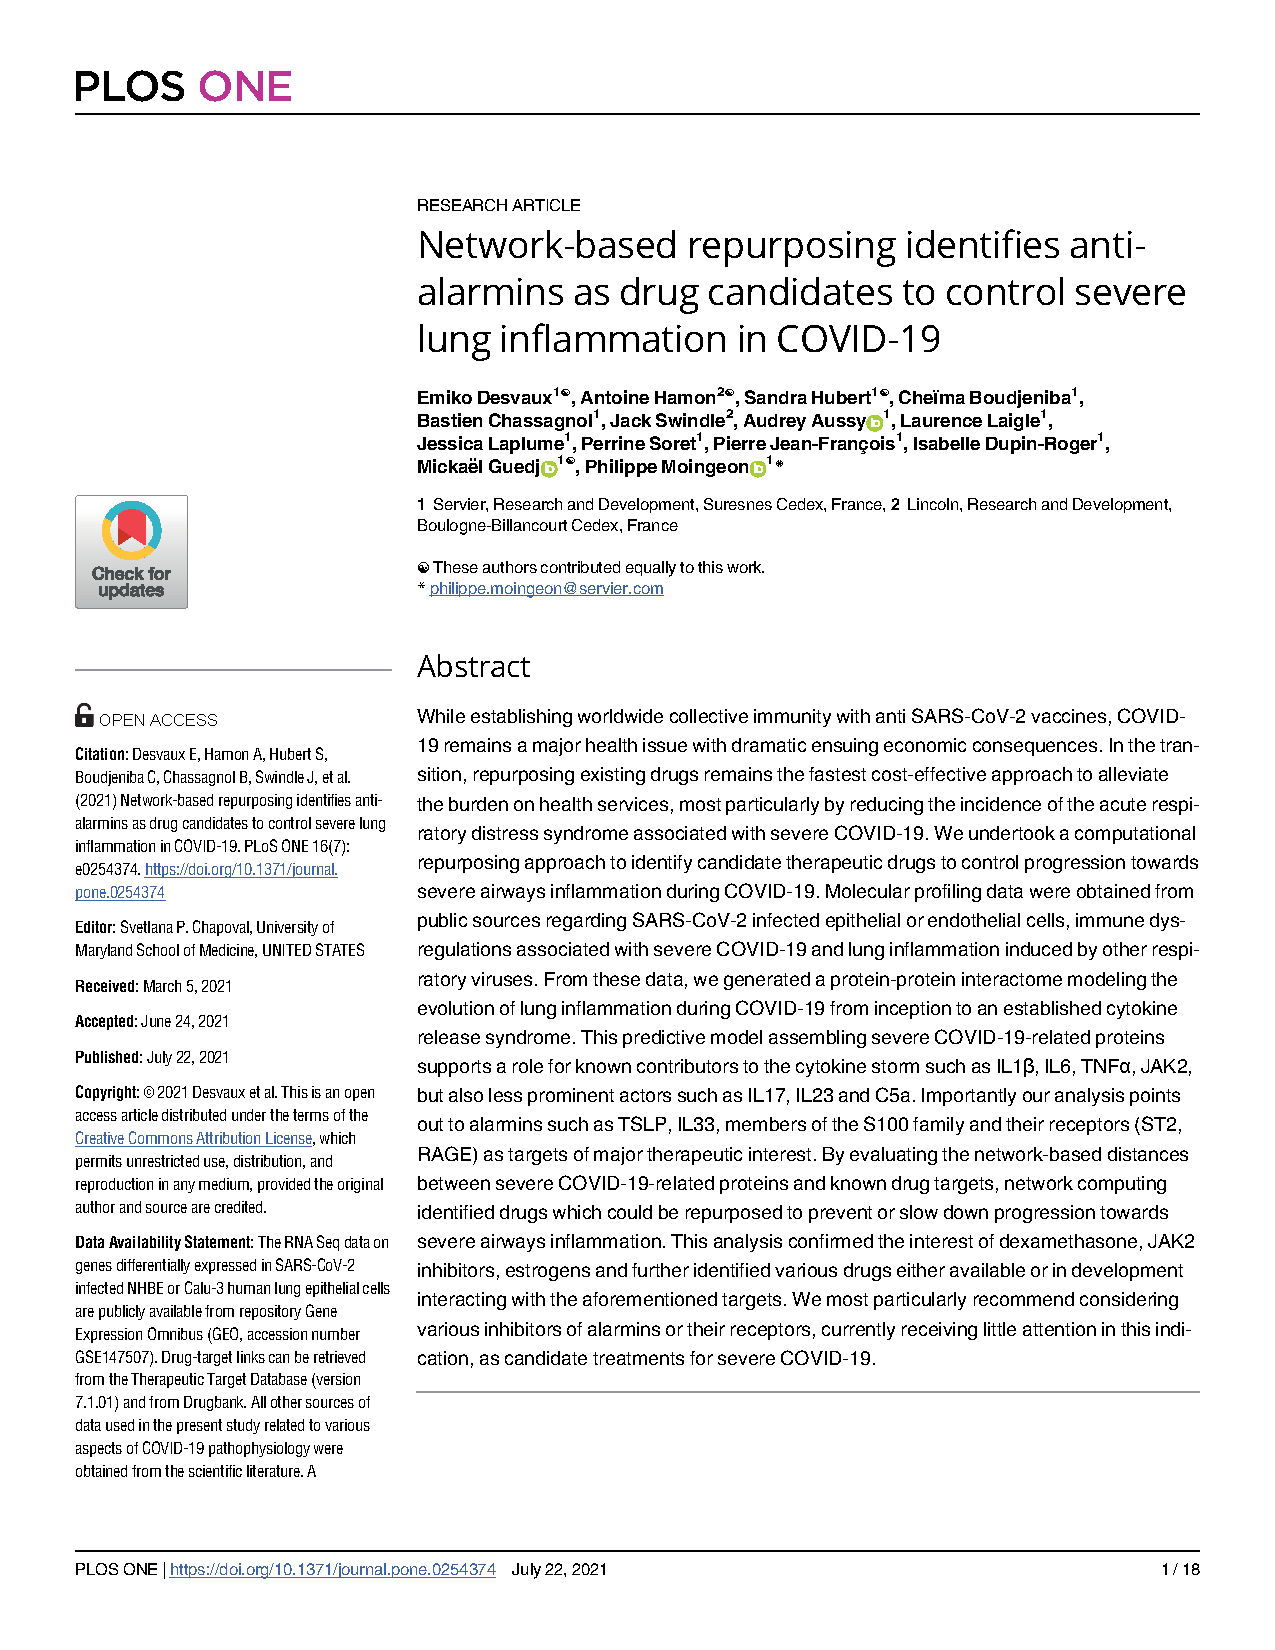
\includepdf[nup=2x1, pages={-}]{repurposing_covid.pdf}

\section{Conclusion}
This repurposing study identified putative drug targets to reduce severe cases of inflammation occurring in patients suffering from COVID-19, including markers involved in cytokine storms and alarmins. In particular, the relevance of our approach has been confirmed by the identification of anti-IL6 and anti-TNF$alpha$ antibodies, such as TSLP, IL33 and S100, as promising targets, and they are currently being used in experimental clinical trials as promising candidates for treating severe cases of COVID-19 (see \autocite{yalcinkehribar_etal21}, \autocite{roth_etal20} and \autocite{idris_etal20}).

Interestingly, we also highlighted the potential therapeutic effect of drugs that received insufficient attention till now for COVID-19 treatment, such as IL17 and IL23 inhibitors \autocite{pacha_etal20}, the C5 complement inhibitor eculizumab \autocite{carvelli_etal20}, and agonists for the thrombopoietin receptor intervening in mitigating thrombocytopenia (when the platelet population, key for tissue clogging, is too low, \autocite{schneider_etal21}). 

In parallel, we highlighted the role of alarmin family proteins (e.g. defensins, HMGB1, IL1$alpha$, IL25, IL33, and S100 proteins, a comprehensive review is proposed in \autocite{yang_etal17}) in COVID-19 lung inflammation and thus suggests resorting to anti-alarmin therapies as a complementary approach to handle severe COVID-19 cases. Last but not least, Topoisomerase 1 inhibitors \autocite{ho_etal20}, currently used as cytotoxic drugs in oncology, were also identified as potential candidates in inhibiting SARS-CoV-2 inflammation and death in animal models. 

Overall, our comprehensive data-driven and agnostic approach enabled to identify disease-related proteins and potential drugs for repurposing in the treatment of severe lung inflammation during COVID-19. Precisely, the combination of several repurposing strategies, namely network-based drug repurposing and Cmap-based analysis, allowed us to prioritise candidate drugs to be investigated for their hypothetical efficacy in mitigating the severe consequences of COVID-19. Retrospectively, it appears that the strategy combining repurposed existing drugs to cure the most severe cases with mRNA vaccines deployed worldwide was an efficient approach to overcome the COVID-19 scourge, as demonstrated in \autocite{yadav_etal}, \autocite{bellera_etal21} and \autocite{taibe_etal22}. 


In this paper, I mostly contribute by retrieving a transcriptomic signature of Covid19-infected lung cells, leveraging the RNASeq expression extracted from Calu-3 and NHBE. To perform these standard differential analyses, we notably capitalise with my PhD partner on our newly industrial and homogenised RNASeq pipeline, see \Cref{chap:transcriptome-workflow} for details. Then, I profit from the same pipeline to homogenise the perturbagen transcriptomic profiles of the Cmap database, ensuring notably to reduce batch and normalisation artefacts between the infected samples and the ones from the molecular profile collection. Finally, I compared several enrichment analyses or distant-metrics scores to assert statistically how similar two gene expression profiles are, providing complementary material to section \texttt{Supportive Cmap-based for drug repurposing} of \autocite{desvaux_etal21}. In our study, it appears that a simple Pearson correlation metric, while making strong naive assumption of linearity between two compared profiles, showcases the most consistent results with respect to the drug-disease links returned by the network-based methodology. 

\section{Perspectives}
\label{sec:perspectives-repositioning}
Given the rather limited set of transcriptomics data available and the small Cmap coverage for repurposable drugs (i.e. only 17$\%$ of molecules in our drug database), results were only used to support the present study. Indeed, among the top network-based drugs, only 2 corticosteroids (betamethasone and hydrocortisone) exhibited a significantly inverted gene expression profile (Cmap score < -0.3) when compared to the Covid-19 gene expression profile.
To that end, the L1000 project is a promising avenue by extending by several orders of magnitude the Cmap expression profiles database. Through the new L1000 technology \footnote{hence named, as this method represents both a 1,000-fold scale-up of the CMap profiling database and only accounts for the expression of \num{1000} key genes}, an experimental high-throughput profiling platform, the large-scale L1000 database embraces a much larger diversity of perturbagen signature profiles, ranging from drugs to genetic manipulations (mostly elicited from Knock out or Knock down experiences) through mutagen factors. While the general principle of treating human cells with different perturbagens is comparable to the Cmap underlying principle, the generation of the L1000 database involves an additional step, since, instead of measuring the expression level of the entire genome, only a subset of \emph{landmark genes} are directly acknowledged, carefully selected such that they are representative of the entire transcriptome and can be used as proxies to infer the expression of remaining genes. Interestingly, \autocite{subramanian_etal17} demonstrate that this protocol compared favourably to RNA sequencing in terms of robustness and accuracy to infer the expression levels of approximately $81\%$ of transcripts coding for proteins, that were not yet directly measured. Ultimately, by taking up to a much larger scale the Cmap compendium, the measured aggregation of dozens of thousands of perturbagen profiles is expected to provide a priceless resource for understanding cellular responses to different stimuli and hereby elucidating novel biological pathways and insights into disease mechanisms, while providing an integrative way to explore shared transcriptomic mechanisms  induced by various treatments, facilitating drug discovery or repositioning (see also their web, user-friendly API, available here \href{https://clue.io/}{clue.io}).


A significant limitation of the methodology devised with Patrimony is the potential loss of meaningful and interpretable biological information, since we fuse diverse datasets, from multiple omics to drug interaction databases, into a single global knowledge graph. Although this initial aggregation step facilitates medical review and validation afterwards, it may compromise the robustness and sensitivity of the analysis due to the integration of disparate and divergent sources of information, an issue already yielded in \Cref{sec:sjogren-extension}. Furthermore, searching for drug similarities and interactions reveal a highly memory- and time-consuming task, primarily due to the high-dimensionality and number of datasets that were integrated in the Patrimony project. By reviewing the recent repurposing literature, I was stunned by the iCell method \autocite{malod-dognin_etal19} to tackle these scalability and integration issues, since iCell was precisely set up to determine clusters of highly co-expressed genes across dissimilar interaction databases.

Briefly, the iCell framework merges three molecular interaction networks (Protein-protein interaction: PPI, Genetic interaction: GI and gene Coexpressions: COEX), all represented as indicator adjacency matrices (symmetric matrices in which an off-diagonal 1 encodes for an existing interaction, 0 otherwise), by projecting them into a smaller subspace of shared cluster of genes. Precisely, these three matrices were simultaneously decomposed into a common matrix $\boldsymbol{G}$, describing gene cluster annotations shared across all networks, and a compressed, omic-specific $\boldsymbol{S}_i$ matrix, showing how gene clusters are related to each other. This decomposition was achieved by minimizing a Multiple Symmetric Non-negative Matrix Tri-Factorization (MSNMTF) objective function.

Since then, this methodology was extended to integrate completely distinct sources of information, firstly in a naive manner, by taking profit of the cluster-indicator matrix returned by iCell as compact and informative input for other biological applications, such as patient clustering and stratification \autocite{xenos_etal23} or inferring new drug-pathway interactions \autocite{malod-dognin_etal23}. \autocite{malod-dognin_etal23} generated new drug repurposing hypotheses to cure severe cases of Covid-19, based on the Graph-regularized Non-negative Matrix Tri-Factorization (GNMTF) method. This algorithm was used to combine the reconstructed and rewired clusters of genes resulting from infected COVID-19 cases, computed with the previously described iCell methodology \footnote{Interestingly, the same two cell lines that we used to retrieve enriched pathways in \autocite{desvaux_etal21}, namely Calu3 and NHBE, were used to that purpose.}, with drug-target interactions (DTIs) and Drug Chemical Similarity (DCS) networks from DrugBank, the latter being represented by its \emph{Laplacian} version (the diagonal degree matrix subtracted to the drug-drug adjacency matrix, in other words a matrix whose diagonal stores the degree vertices, and the off-terms pairwise interactions, with a -1 positively coding for a direct connection). Precisely, the main idea was to retrieve the low-dimensional gene clusters-drug interaction matrix, resulting from both a matrix factorisation with an additional regularisation term to account for the known structure of the DCS network, which predicts the best the global drug-target interaction matrix while projected into a much lower dimensional space (see \autocite[Eq 1.]{malod-dognin_etal23} for the explicit optimisation problem). Ultimately, the new drug-target interaction matrix, supposedly with higher completion as inferred from disease-specific omics, was reconstructed to predict individual drug-target interactions. Indeed, each entry in the reconstructed matrix stands for an \emph{association score}, supposed to be significant if the predicted drug-target interaction scores higher than the mean of existing interactions. \autocite{xenos_etal23} implements a novel Non-negative Matrix Tri-Factorization (NMTF) strategy to overcome the lack of genetic samples (five samples make up the cohort) to identify novel disease-related genes for antithrombin resistance, since \acrshort{gwas}, while relevant to find disease-associated variants for common diseases, are not suited to rare diseases due to the sparsity of genetic data. And precisely, matrix factorisation techniques can deal with low sample size by integrating prior knowledge and combining different types of biological and medical data.Precisely, the NMTF method was used to integrate four different data types: germline mutations, protein-protein interactions (PPIs), coexpressions (COEXs) and genetic interactions (GIs), the last three being summarised into an indicator matrix $\boldsymbol{G}$ in which hard assignment to a gene cluster is indicated by a 1, 0 otherwise. Then, the genetic patient information matrix $\boldsymbol{M}$ is simultaneously decomposed into the product of three lower dimensional factors, $\boldsymbol{P}$, $\boldsymbol{S}$ and $\boldsymbol{G}$; the latter, storing the $k_1$ gene clusters, being the standard output of the iCell methodology and $\boldsymbol{P}$ storing the $k_2$ patient clusters (see \parencite[Eq.1]{xenos_etal23} for details).

This heuristic method to fuse heterogeneous data entities was further extended to capture in an unified framework all systematic interactions while providing gene and patient clusters and supplying drug target candidates (see \Cref{subfig:icell-extended} for details), with respectively applications to Covid-19 repurposing again \autocite{zambrana_etal21}, cancer stratification to generate personalised treatment \autocite{gligorijevi_etal15} or an ongoing work to determine Parkinson’s trajectories through multiple single-cell RNA-seq time points \autocite[Poster ID: 8328, session P236-M]{PosterECCB2022}. 
These matrix factorisation methods embody a new powerful way-of-thinking to add in the computational toolbox. 

To conclude, by explicitly incorporating interactions across multiple biological entities and systems in an integrated way, thus keeping the mechanistic biological interpretation and facilitating prior knowledge integration, these approaches have the potential to bridge the gap between powerful yet less biologically interpretable and robust AI-based models and more standard statistical methods that struggle with high-dimensional datasets, particularly in the presence of a limited number of replicates. 


However, the methods described earlier are not well-suited for identifying causal genes and reconstructing the chronological sequence of genes involved in pathway signalling. In other words, they may not effectively distinguish between downstream resulting phenotypes and upstream activation events in biological processes, since the inferred graphs are not directed. In this regard, Bayesian networks and their natural extension to Causal networks appear to be particularly well-suited for capturing complex and mechanistic interactions of biological phenomena, and such in their entirety.

For instance, the study conducted by \autocite{li_etal19}, Bayesian networks were used to infer pathways specifically involved in Systemic Lupus Erythematosus (SLE), from a cohort of 1760 SLE patients. Of note, the analysis identified and confirmed the significance of both the JAKSTAT and the Interferon signature, while capitalising on both prior knowledge and novel inferred interactions. Precisely, the pipeline to infer the structure of Bayesian networks comprised three main steps: first, co-expression networks were constructed using the R WGCNA package, returning 3 gene modules highly correlated to the phenotype, encompassing 431 differentially expressed genes. Second, text mining was employed to uncover literature-based gene pairwise connections. Third, both observational data (transcriptomic expression) and prior edges were combined to generate the Bayesian networks: 
\begin{enumerate}
\item  Random graphs were initially created, by integrating the edges inferred through text mining.

\item Subsequently, the igraph package was utilized to remove \emph{bidirectional edges} and \emph{cycles} in the graph. Indeed, one of the primary limitations of Bayesian networks is that they are restricted to the space of Directed Acyclic Graphs (DAGs), which makes them less valuable for describing positive or negative feedback regulation loops.

\item A score-based method from the bnlearn package, employing a hill-climbing algorithm to maximise the likelihood of the generated network structure, was then used to generate an \emph{ensemble model} composed of 100 graphs, in which edges appearing with low frequency were discarded.
\end{enumerate}
A similar process was used in \autocite{mostafavi_etal18}, to build a molecular network of the aging human frontal cortex, and identifies specifically the pathways leading to Alzheimer’s degeneracy and cognitive decline. \autocite{mostafavi_etal18} includes an additional validation step to highlight key driver genes, through direct interventions, in the form of knock-outs to directly silence the expression of genes one by one, and evaluated by conducting standard ANOVA analysis.

However, instead of integrating causal information posterior to the Bayesian network construction, it is also possible to directly combine interventional and observational information when learning the structure of Bayesian networks. We already discuss a possible framework to do so in \Cref{chap:general-perspectives}, in relation with paper \autocite{rau_etal13}. An alternative approach, in the absence of interventional datasets, is to integrate biological causal prior information. For example, by incorporating the knowledge that DNA nodes should precede RNA nodes, which in turn should be parents of protein nodes, following the central biological paradigm (see Section \ref{sec:gene-protein}). This strategy was demonstrated in \autocite{gruber_etal16} using the proprietary $\text{REFS}^{\text{TM}}$ causal inference engine, where they combined transcriptomic data, clinical features and treatment annotations in an ensemble model of 256 Bayesian networks with \num{30084} variables. The goal was to identify severe pathways involved in myeloma severity and identify patient subpopulations that would benefit most from stem cell transplantation treatment. The RIMBANET algorithm was also used to distinguish simple correlations from causal relations by leveraging DNA-based variations (expression quantitative trait loci, eQTL, or SNP, for single nucleotide polymorphisms), respectively revealing unexplored interconnections between lipid metabolism and glucose regulation pathways in type 2 diabetes \autocite{cohain_etal21} and identifying key regulators of Alzheimer’s disease \autocite{beckmann_etal20}.

However, it is important to note that the performance of Bayesian networks is partly hindered by their lack of scalability to high-dimensional datasets (the sampling space of possible causal node orderings grows exponentially with the number of variables), the strong assumptions they make on the distribution of the datasets (most Bayesian algorithms were developed to accommodate either discretised or Gaussian-shaped distributions), and their high sensitivity to even minor alterations or noise present in the samples.

\newpage 
\begin{figure}
     \centering
     \begin{subfigure}[t]{0.8\textwidth}
         \centering
         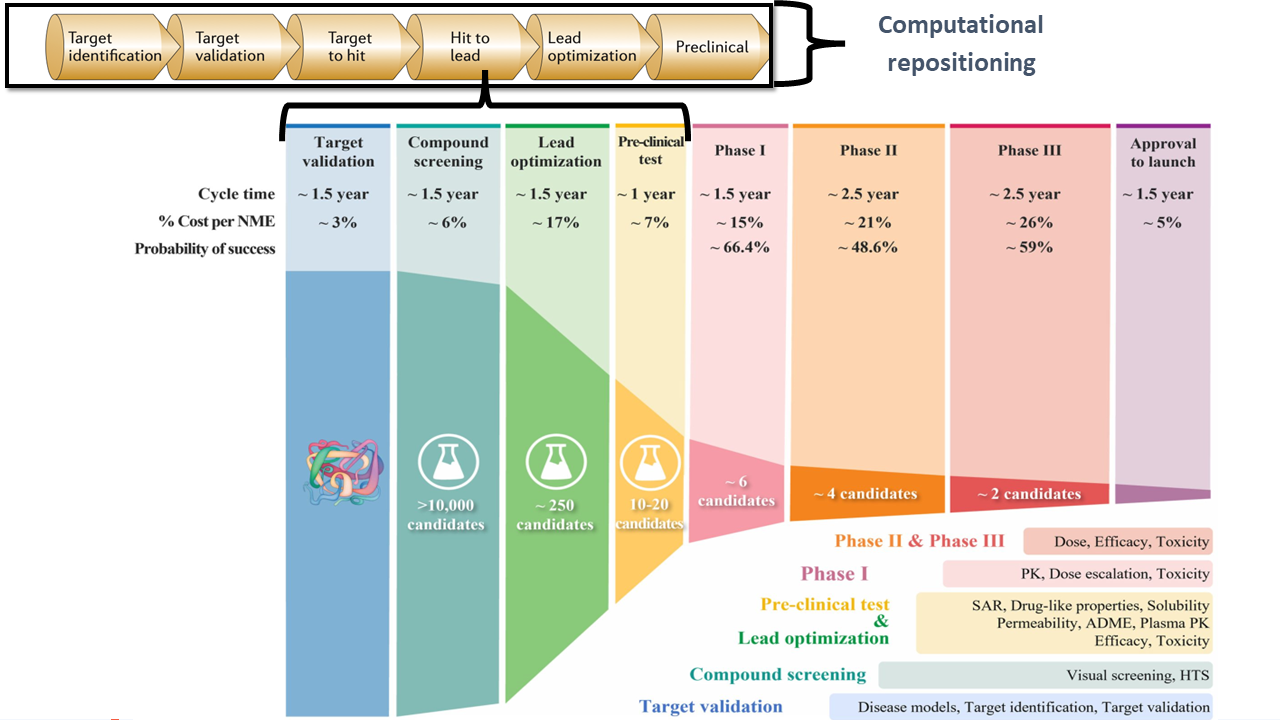
\includegraphics[width=\textwidth]{figures/repurposing/drug_development_pipeline.png}
         \caption[\textbf{Illustration of the \enquote{valley of death} in drug-development cycle}]{We detail here the main stages of the drug-development life cycle as well as their averaged duration, capitalised costs and the probability of failure highlighted as an \enquote{attrition funnel} diagram, as reproduced from \autocite[Fig.1]{philippe22} (see also \href{https://www.linkedin.com/posts/bigidea_great-image-posted-by-alex-telford-on-probability-activity}{Attrition rates for cancer drugs} for details). We additionally detailed the main steps of the exploratory clinical phase, as enumerated in \autocite{hughes_etal11}.}
         \label{subfig:drug-pipeline}
     \end{subfigure}
     \vfill
     \begin{subfigure}[p]{0.8\textwidth}
         \centering
         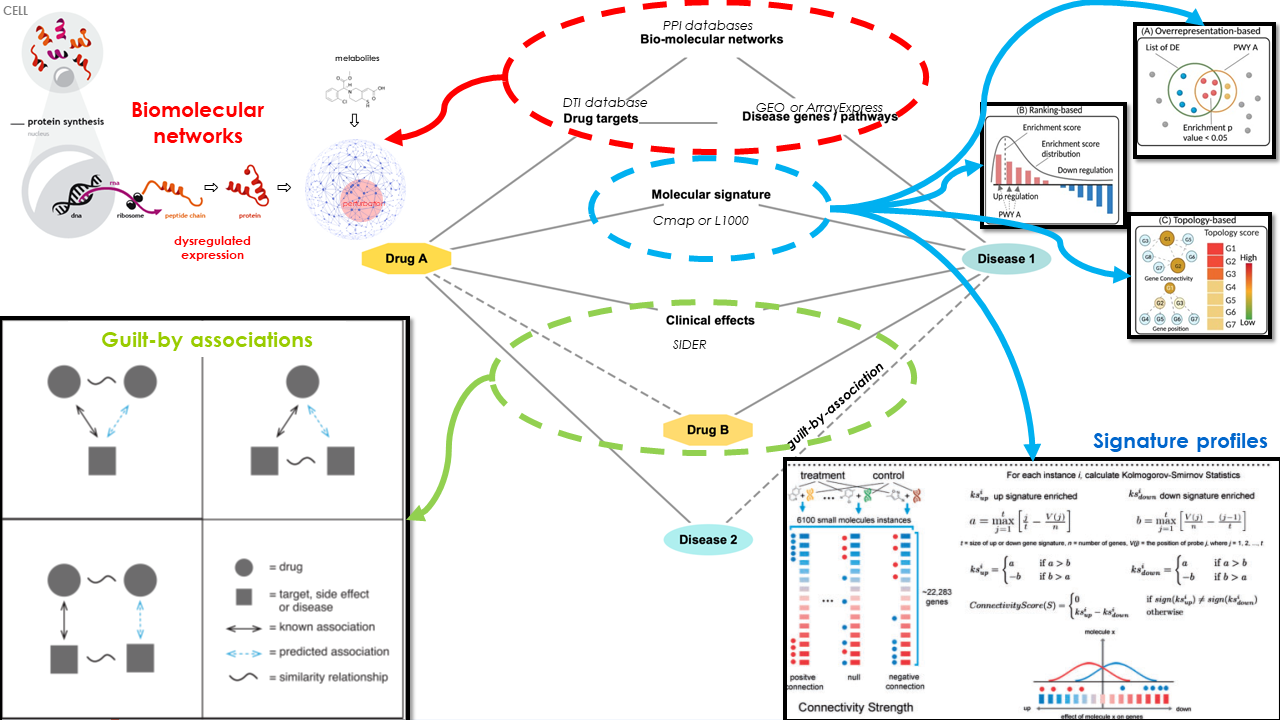
\includegraphics[width=\textwidth]{figures/repurposing/repositioning_strategies.png}
         \caption[\textbf{Main computational repositioning strategies implemented in internal Patrimony computational platform.}]{We mostly used three computational approaches to identify novel drug-disease-gene paired interactions: \textcolor{red}{a) First approach consists of reconstructing molecular networks, using several biological entities, combine them with drug target interaction databases to ultimately predict the effect of a new treatment in a systematic manner. \textcolor{blue}{The second approach matches transcriptomic profiles between perturbagens and disease phenotype, the general idea being that an opposite signature should revert the dysregulated mechanism towards its healthy state. The top 3 panels describe several association metrics, from \autocite[Fig.1]{zhao_rhee23}, while the bottom panel, from \autocite[Fig.1]{musa_etal17}, displays in a visual, user-friendly way the principle underlying the Cmap enrichment score.} \textcolor{green}{Various guilt-by-association strategies in computational pharmacology, reproduced from \autocite[Fig.3]{hodos_etal16}.}}}
\label{subfig:repositioning-strategies}
     \end{subfigure}
     \begin{subfigure}[b]{0.4\textwidth}
         \centering
         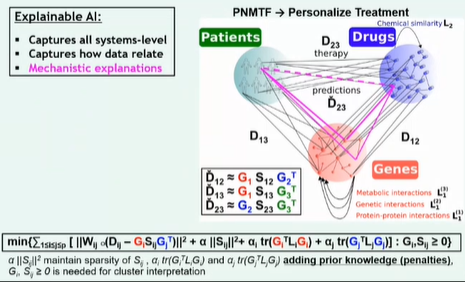
\includegraphics[width=\textwidth]{figures/repurposing/icell_extended_framework.png}
         \caption[\textbf{NNMF extended to integrate multiple entities.}]{Final extension of NNMF, termed PNMTF for Patient Non-negative Matrix Tri-Factorization, covers three distinct sources: drug-target interactions, gene co-expression, and patient clinical features. Within the same framework, the versatility of the tool enables to perform simultaneously hard clustering of patients and genes, while suggesting new drug repurposing strategies, from a reproduction of \autocite{malod-dognin_etal23}.}
         \label{subfig:icell-extended}
     \end{subfigure}  
     \hfill
     \begin{subfigure}[b]{0.4\textwidth}
         \centering
         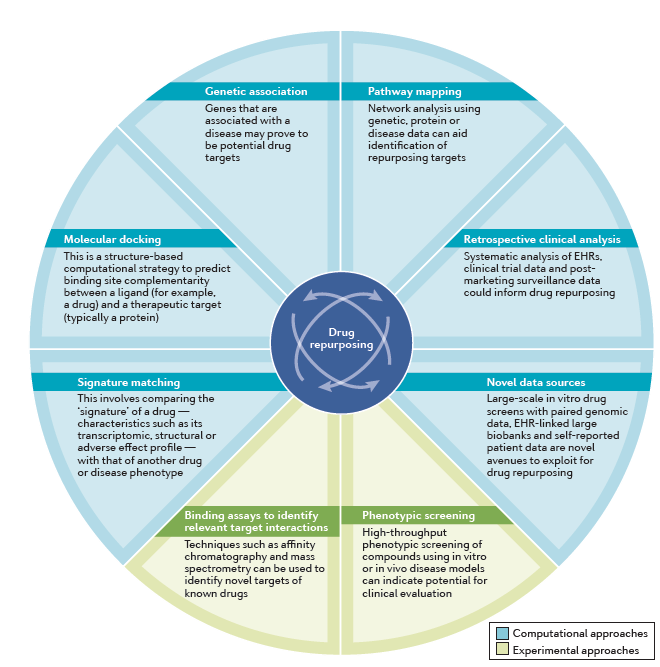
\includegraphics[width=\textwidth]{figures/repurposing/repositioning_strategies_general.png}
         \caption[\textbf{Drug repurposing strategies}]{Various computational approaches can be used individually or in combination to merge large-scale and highly heterogeneous datasets and generate hypotheses for drug repositioning, from a reproduction of \autocite[Fig. 1]{pushpakom_etal19}. These approaches are frequently utilized alongside traditional experimental techniques, which themselves demand significant computational resources to manage the increasing throughput analysis.}
         \label{subfig:repositioning-strategies-general}
     \end{subfigure}  
    \caption{Infographic 2) of Appendix C, detailing several computational repurposing methods}
    \label{fig:infographic-repurposing}
\end{figure}






